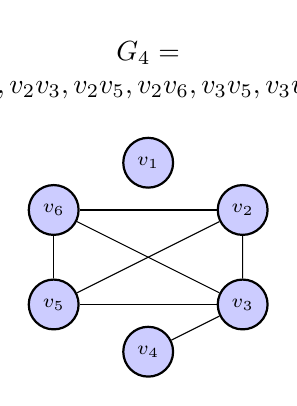
\begin{tikzpicture}
  [scale=.6, auto=left, 
   vertex/.style={circle, fill=blue!20, draw=black, thick, inner sep=2pt, minimum size=18pt}]

  \node[vertex] (n1) at (2,4) {$\scriptstyle v_1$};
  \node[vertex] (n2) at (4,3) {$\scriptstyle v_2$};
  \node[vertex] (n3) at (4,1) {$\scriptstyle v_3$};
  \node[vertex] (n4) at (2,0) {$\scriptstyle v_4$};
  \node[vertex] (n5) at (0,1) {$\scriptstyle v_5$};
  \node[vertex] (n6) at (0,3) {$\scriptstyle v_6$};

  \foreach \from/\to in {n3/n4,n2/n3, n2/n5, n2/n6, n3/n5, n3/n6, n5/n6}
    \draw (\from) -- (\to);

  \node[anchor=south, yshift=0.3cm] at (n1.north) {%
    \makebox[0pt][c]{%
      $\begin{array}{c}
        G_4=\\
        (V,\{v_3v_4, v_2v_3, v_2v_5, v_2v_6, v_3v_5, v_3v_6, v_5v_6\})
      \end{array}$%
    }%
  };
\end{tikzpicture}
